% !TEX encoding = UTF-8 Unicode
% !TEX root = ../thesis.tex
% !TEX spellcheck = en-US
%%=========================================



\chapter{Background}

% \section{Glossary?}

\section{Augmented Reality}
% (Jentoft, 2020) AR can be defined as a system that fulfills three basic features: a combination of real and virtual worlds, real-time interaction, and accurate 3D registration of virtual and real objects.


% \subsection*{Augmented Reality}
Augmented Reality (AR) describes the use of computer technology to generate an audio-visual experience combining real-world impressions with computer generated graphics, and, \textit{essentially}, the ability to interact seamlessly within both domains. Ever since its infancy medical usage of AR technology has been envisioned as a great potential. The idea of x-ray vision is seen both in science fiction and in genuine research dating all the way back to the 1930s when H. Steinhaus explored ways to visualize metal pieces inside the body \citep{Sielhorst2008}. There is now substantial interest in the use of AR within a wide array of medical fields as well as in industry and education. As an emerging technology there is still much research needed, and great leaps in hardware, software and sensor capabilities are bound to happen in the near future. Already AR shows promising results in both surgical settings and in education \citep{Singh2013}.


\subsection*{Disambiguation of some acronyms}\label{chap:armrxr}
As a new field, this field suffers from naming disagreements. This is a confusing reality which needs to be addressed. There are differing view of what each acronym refers to, and even what they stand for. I will overlook most of this discussion, and simply explain what is meant by each acronym in the scope of this project.

\paragraph*{VR}\label{para:vr} Virtual Reality, is enclosed experiences which completely surrounds the user within a computer generated world. This is a generally uncontroversial term and will be used for applications running on devices like the Oculus Rift and the HTC Vive.

\paragraph*{AR}\label{para:ar} Augmented Reality, exercises which implement a see-through effect to display 3D visuals on top of the real-world. The idea of holograms is a good stand-in for the effect of AR. This is the term which will be most used in this project. 

\paragraph*{MR}\label{para:mr} Mixed Reality, anything within the spectrum between reality and pure visual 3D graphics, which blends computer generated visuals and reality. While the term has been in use since it was coined by \citet{Milgram1994}, it has in recent years been strongly associated with Microsoft, and in this project the term MR will generally only be used as a reference to Microsoft's products or concepts. The term is also used by some as a subset of \nameref{para:ar}, so in conclusion it is a somewhat controversial term. 


\paragraph*{XR}\label{para:xr} Extended Reality, much like \nameref{para:mr} this includes the whole spectrum of experiences blurring the line between the real and the virtual. However it does not have the Microsoft taint, nor the confusion of that term. And thus it is a more acceptable term, and it is what will be used here to describe the spectrum.


\section{Graphics and Rendering}

\subsection*{Models}

Three dimensional data can be stored and visualized in a number of ways, and the way a graphical application like Nevrolens does it is very different from the ways of medical applications. Within medicine volumetric data is common, as it is just as important what's inside the model as what's outside. In conventional graphics 3D models are built up of 2D polygons which added up forms a 3D structure, this reduces rendering time while keeping the outside structure of the model intact. \autoref{fig:lowpolyratbrain} show a model with about 15 thousand polygons. 

The process of generating polygonal models from volumetric models is quite complex, \citet{Elden2017} writes about this process in some detail, which can be found in \autoref{chap:elden}. This is the model used in this research project though the model had to be simplified further to about 300,000 triangles, to run decently on the HoloLens 2.  

This research also makes use of the medical data to visualize the brain segmentations inside the volume. The is three dimensional data captured from MRI with a resolution of 512x1024x512 voxels and a voxel size of 39 $\mu$m. This results in a 0.5GiB texture asset in the application memory, and rendering of 1024x1024 slices of the volume.

\begin{figure}[ht]
    \centering
    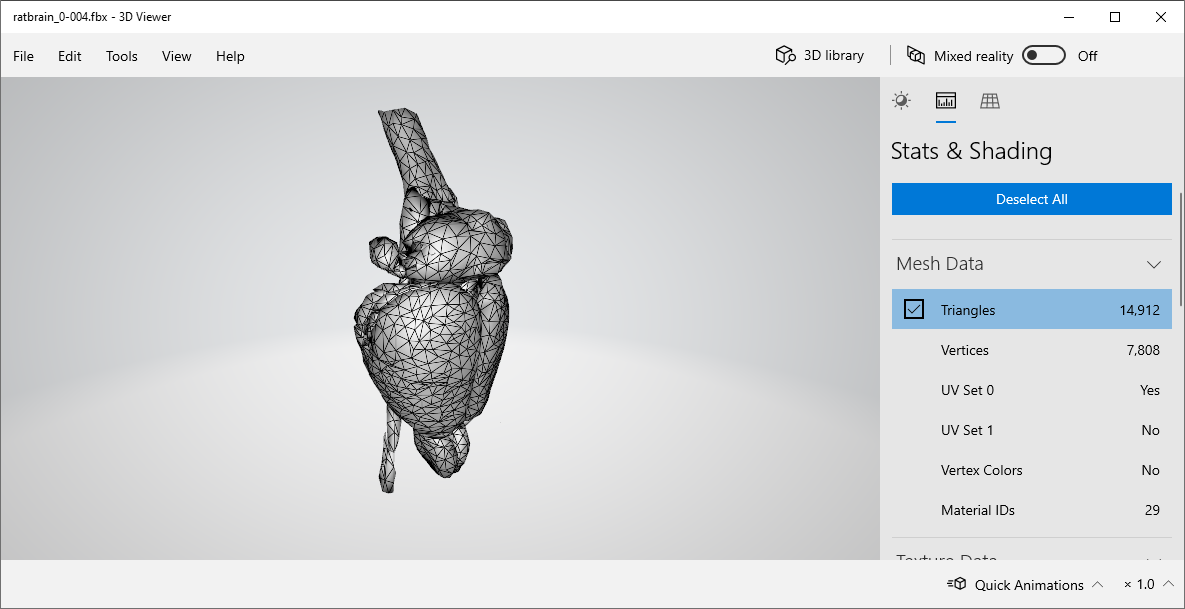
\includegraphics[width=\textwidth]{fig/ratbrain_lowpoly}
    \caption{Wireframe view of the low resolution rat brain in Microsoft 3D Viewer. The triangles are clearly distinguishable, in total there is 14,912 triangles in this model. }
    \label{fig:lowpolyratbrain}
\end{figure}


% surface vs volume model

\subsection*{Colors}

% rgb hsv

\begin{wrapfigure}{r}{0.45\textwidth}
    \begin{center}
        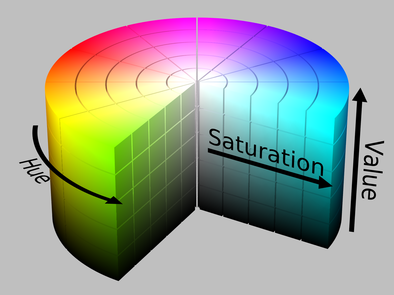
\includegraphics[width=0.42\textwidth]{fig/hsv_illustration}
    \end{center}
    \caption{HSV color model represented cylindrically.}
\end{wrapfigure}

Within computer graphics colors are generally encoded by their component primary color values in separate channels, this is called RGB for red, green and blue. This is the basis for most color models used on computers. The RGB color model is naturally used widely in this project, and will not be explained further. There is however another less common color model used in this project which has some useful properties worth exploring. 
This is the HSV color model. The different channels are hue, saturation, and value. The hue is simply the color based on a traditional color wheel, this means that the color will periodically repeat starting with red on hue=0, green on hue=0.33 and green on hue=0.67. The saturation is how "colorful" the color is, there 0 is a gray-scale and 1 is completely colored. The value is sometimes also called light or brightness, where 0 is black and 1 is again completely colored.
% This color model is designed to be more intuitive for human use and also 


\subsection*{Transformation}\label{chap:transformation}



% todo affine transformation


% \subsection*{Rasterization, Polygons and 3D models}

% {
%     \color{BrickRed}
%     I feel that there is some misunderstanding about what a 3D model is.
%     Maybe go in-depth about what I mean by 3D model. I have probably already used the term for different things.
% }
% Three-dimensional graphics 
% The conversional rendering pipe-line

\section{Neuroanatomy}

The study of neuroanatomy is concerned with the structural organization of the nervous system. This primarily means the brain and its structures, and is what this project will focus exclusively on.
Within the study of neuroanatomy, the use of macroscopical brain dissections have long been the conventual practice for teaching the organization of the structures in the brain. Requiring cadavers and the single use of their brain, this method is highly resource intensive and has limited scalability. In addition, there are concerning ethical challenges with the use of animals in research. 

% \subsection*{Ethics of dissection}\label{chap:ethics}

\subsection*{The Waxholm Space Atlas of the Sprague Dawley Rat Brain}\label{chap:ratbrain}

% {
%     \color{BrickRed}
% https://www.nitrc.org/projects/whs-sd-atlas
% \begin{itemize}
%     \item What is a atlas
%     \item WHS and ratbrain is open, used and developed by NTNU St Olavs and UiO 
%     \item Waxholm Space Atlas of the Sprague Dawley Rat Brain 
%     \item Discuss difference between graphical 3D model and 3D atlas
% \end{itemize}
% }


%  In this pursuit we will also make use of high-resolution 3D imagery of a rat brain (see \autoref{chap:ratbrain}).  

This project makes use of high-resolution 3D-models of a rat brain. This brain model has been captured and manually delineated\footnotemark[1] by a collaboration between research groups at the University of Oslo and NTNU, and is in fact a highly accurate volumetric representations of the rat brain. This model is an open access community resource, intended as a free tool for education and research\footnotemark[2]. Within the convectional rasterization rendering pipe-line of Nevrolens, a geometric asset derived from this volumetric model is naturally used. 

\footnotetext[1]{Delineation refers to the process of clearly defining different structures in the brain into separate namable parts.}
\footnotetext[2]{https://www.nitrc.org/projects/whs-sd-atlas}

The model is referred to as \textit{The Waxholm Space Atlas of the Sprague Dawley Rat Brain}. That means a atlas of the \textit{Sprague Dawley} rat breed defined in Waxholm Space. I will briefly explain what a brain atlas is and what Waxholm space is. 


\subsubsection*{Brain Atlas}\label{chap:atlas}

A brain atlas is a composite representation based on one or more datasets of a given brain. An atlas generally has the function of highlighting some specified aspects and relations in the brain, and is a convectional tool in neuroscientific research \citep{Toga2000_AtlasBasics}. The convectional atlas is based on micrometer scale sliced sections in the brain, effectively creating two-dimensional layers through the brain. While functional, this "turns the brain into a book". Three-dimensional digital atlas are however relative newcomer on the neuro-imagery scene, by employing magnetic resonance imaging (MRI) and diffusion tensor imaging (DTI) the resulting atlases are complete volumetric representation of the subject brain \citep{WaxholmRatBrain2014}. 

This volumetric model is the basis for the delineated 3D-model used in Nevrolens.


\subsubsection*{Waxholm Space}\label{chap:whs}
\begin{wrapfigure}{r}{0.45\textwidth} 
    \centering
    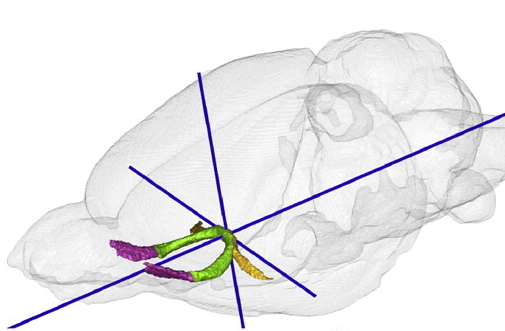
\includegraphics[width=0.40\textwidth]{fig/waxholmspace2}
    \caption{\raggedright Waxholm Space \citep{WaxholmRatBrain2014}}
    \label{fig:waxholmspace}
\end{wrapfigure}

Waxholm Space (WHS) is a vector space defined as a standard reference space for the mouse brain and the rat brain \citep{WaxholmWithSimpleAbstract2013}. Its use as a coordinate system simplifies interoperability across atlases. It was developed by International Neuroinformatics Coordinating Facility (INCF) for the mouse brain, and has further been implemented in the rat brain by \citet{WaxholmRatBrain2014}. The following is the formal definition of WHS:


%  International Neuroinformatics Coordinating Facility (INCF) Digital Atlasing Project
\begin{quote}
\textit{
The coordinate system for WHS is defined as a continuous Cartesian system with the origin in the brain determined by 
\begin{itemize}
    \item the anterior commissure (AC) at the intersection between the mid sagittal plane,
    \item a coronal plane passing midway (rostro-caudal) through the anterior and posterior branches of AC, and
    \item a horizontal plane passing midway through the most dorsal and ventral aspect of the AC.
\end{itemize}
}
\citet{WaxholmSpaceAndMouseBrain2011}
\end{quote}

\noindent
\autoref{fig:waxholmspace} visualizes the axes through origin of WHS in the brain of a rat. Within the scope of this project WHS will be the local space of the rat brain model implemented in Nevrolens.




\section{Equipment}

\subsection*{HoloLens 2}\label{chap:hololens2}

\begin{figure}[ht]
    \centering
    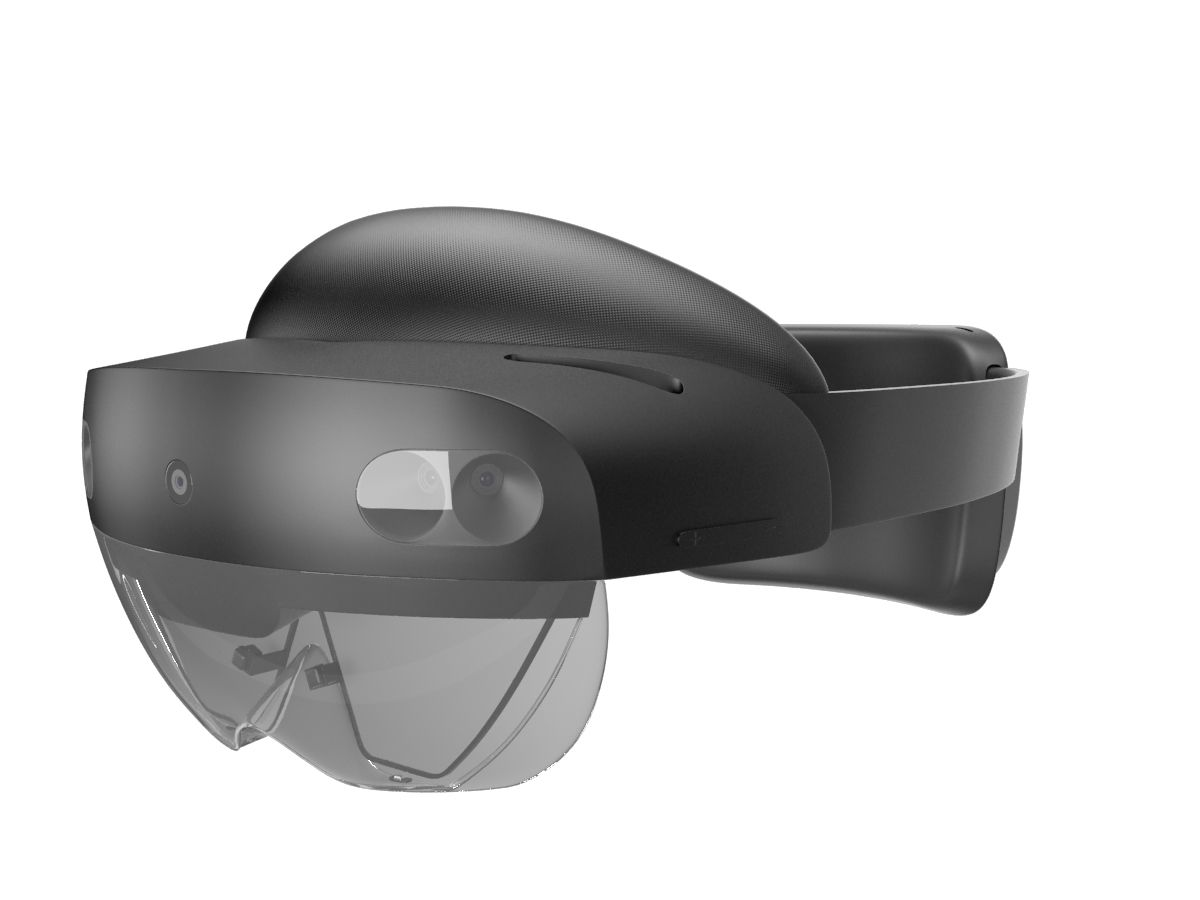
\includegraphics[width=0.4\textwidth]{fig/hololens2}
\end{figure}

HoloLens 2 is the second iteration of Microsoft immersive headset line. It uses an ARM-based computing unit, running a custom holographic version of Windows 10 for ARM. This enables the HoloLens 2 to produce high quality graphics while being very power efficient. It was announced in early 2019, with a limited release on November 7, 2019. It is however jet, as of writing, not publicly available and could be considered a limited industrial product.
As the technology stands today, HoloLens 2 is the most complete augmented reality device on the marked, with interaction features like hand tracking and eye tracking in combination with the most immersive display technology in any AR HMD. This makes it a natural device choice for developing AR applications with today. \author{fig:specshololens2}
Very helpfully the HoloLens 2 has on-board screen capturing tools and the option to live preview the video feed from the Windows Device Portal. These features have helped greatly both in user testing and in demonstration the application.

\begin{figure}[ht]
    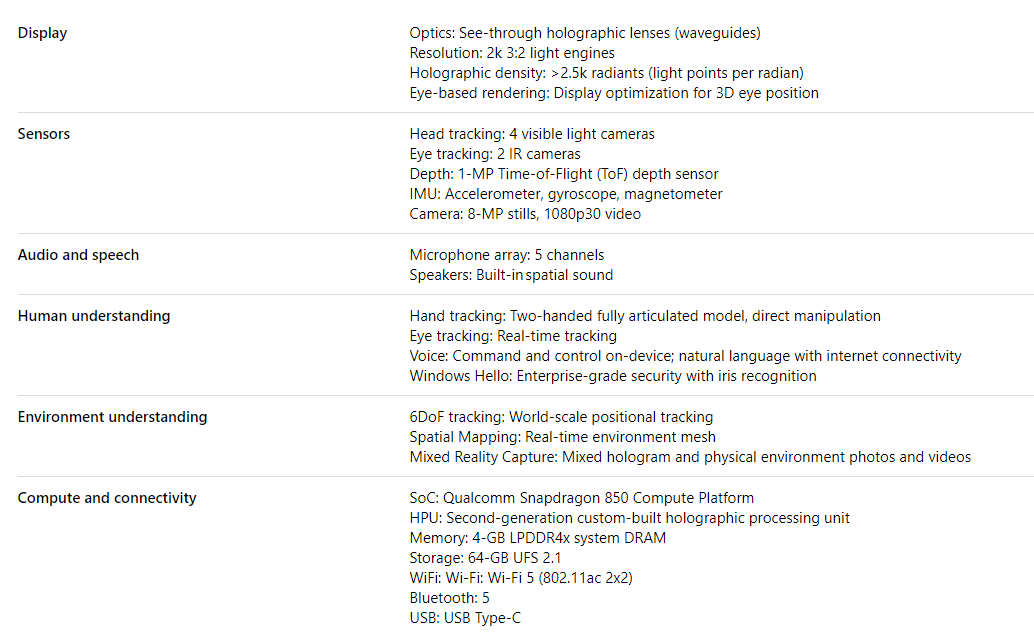
\includegraphics[width=\textwidth]{fig/hololens2specs}
    \caption{Specifications for the HoloLens 2}
    \label{fig:specshololens2}
\end{figure}




\section{Software Tools}\label{chap:tools}


\subsection*{Unity}\label{chap:unity}

\begin{figure}[ht]
    \centering
    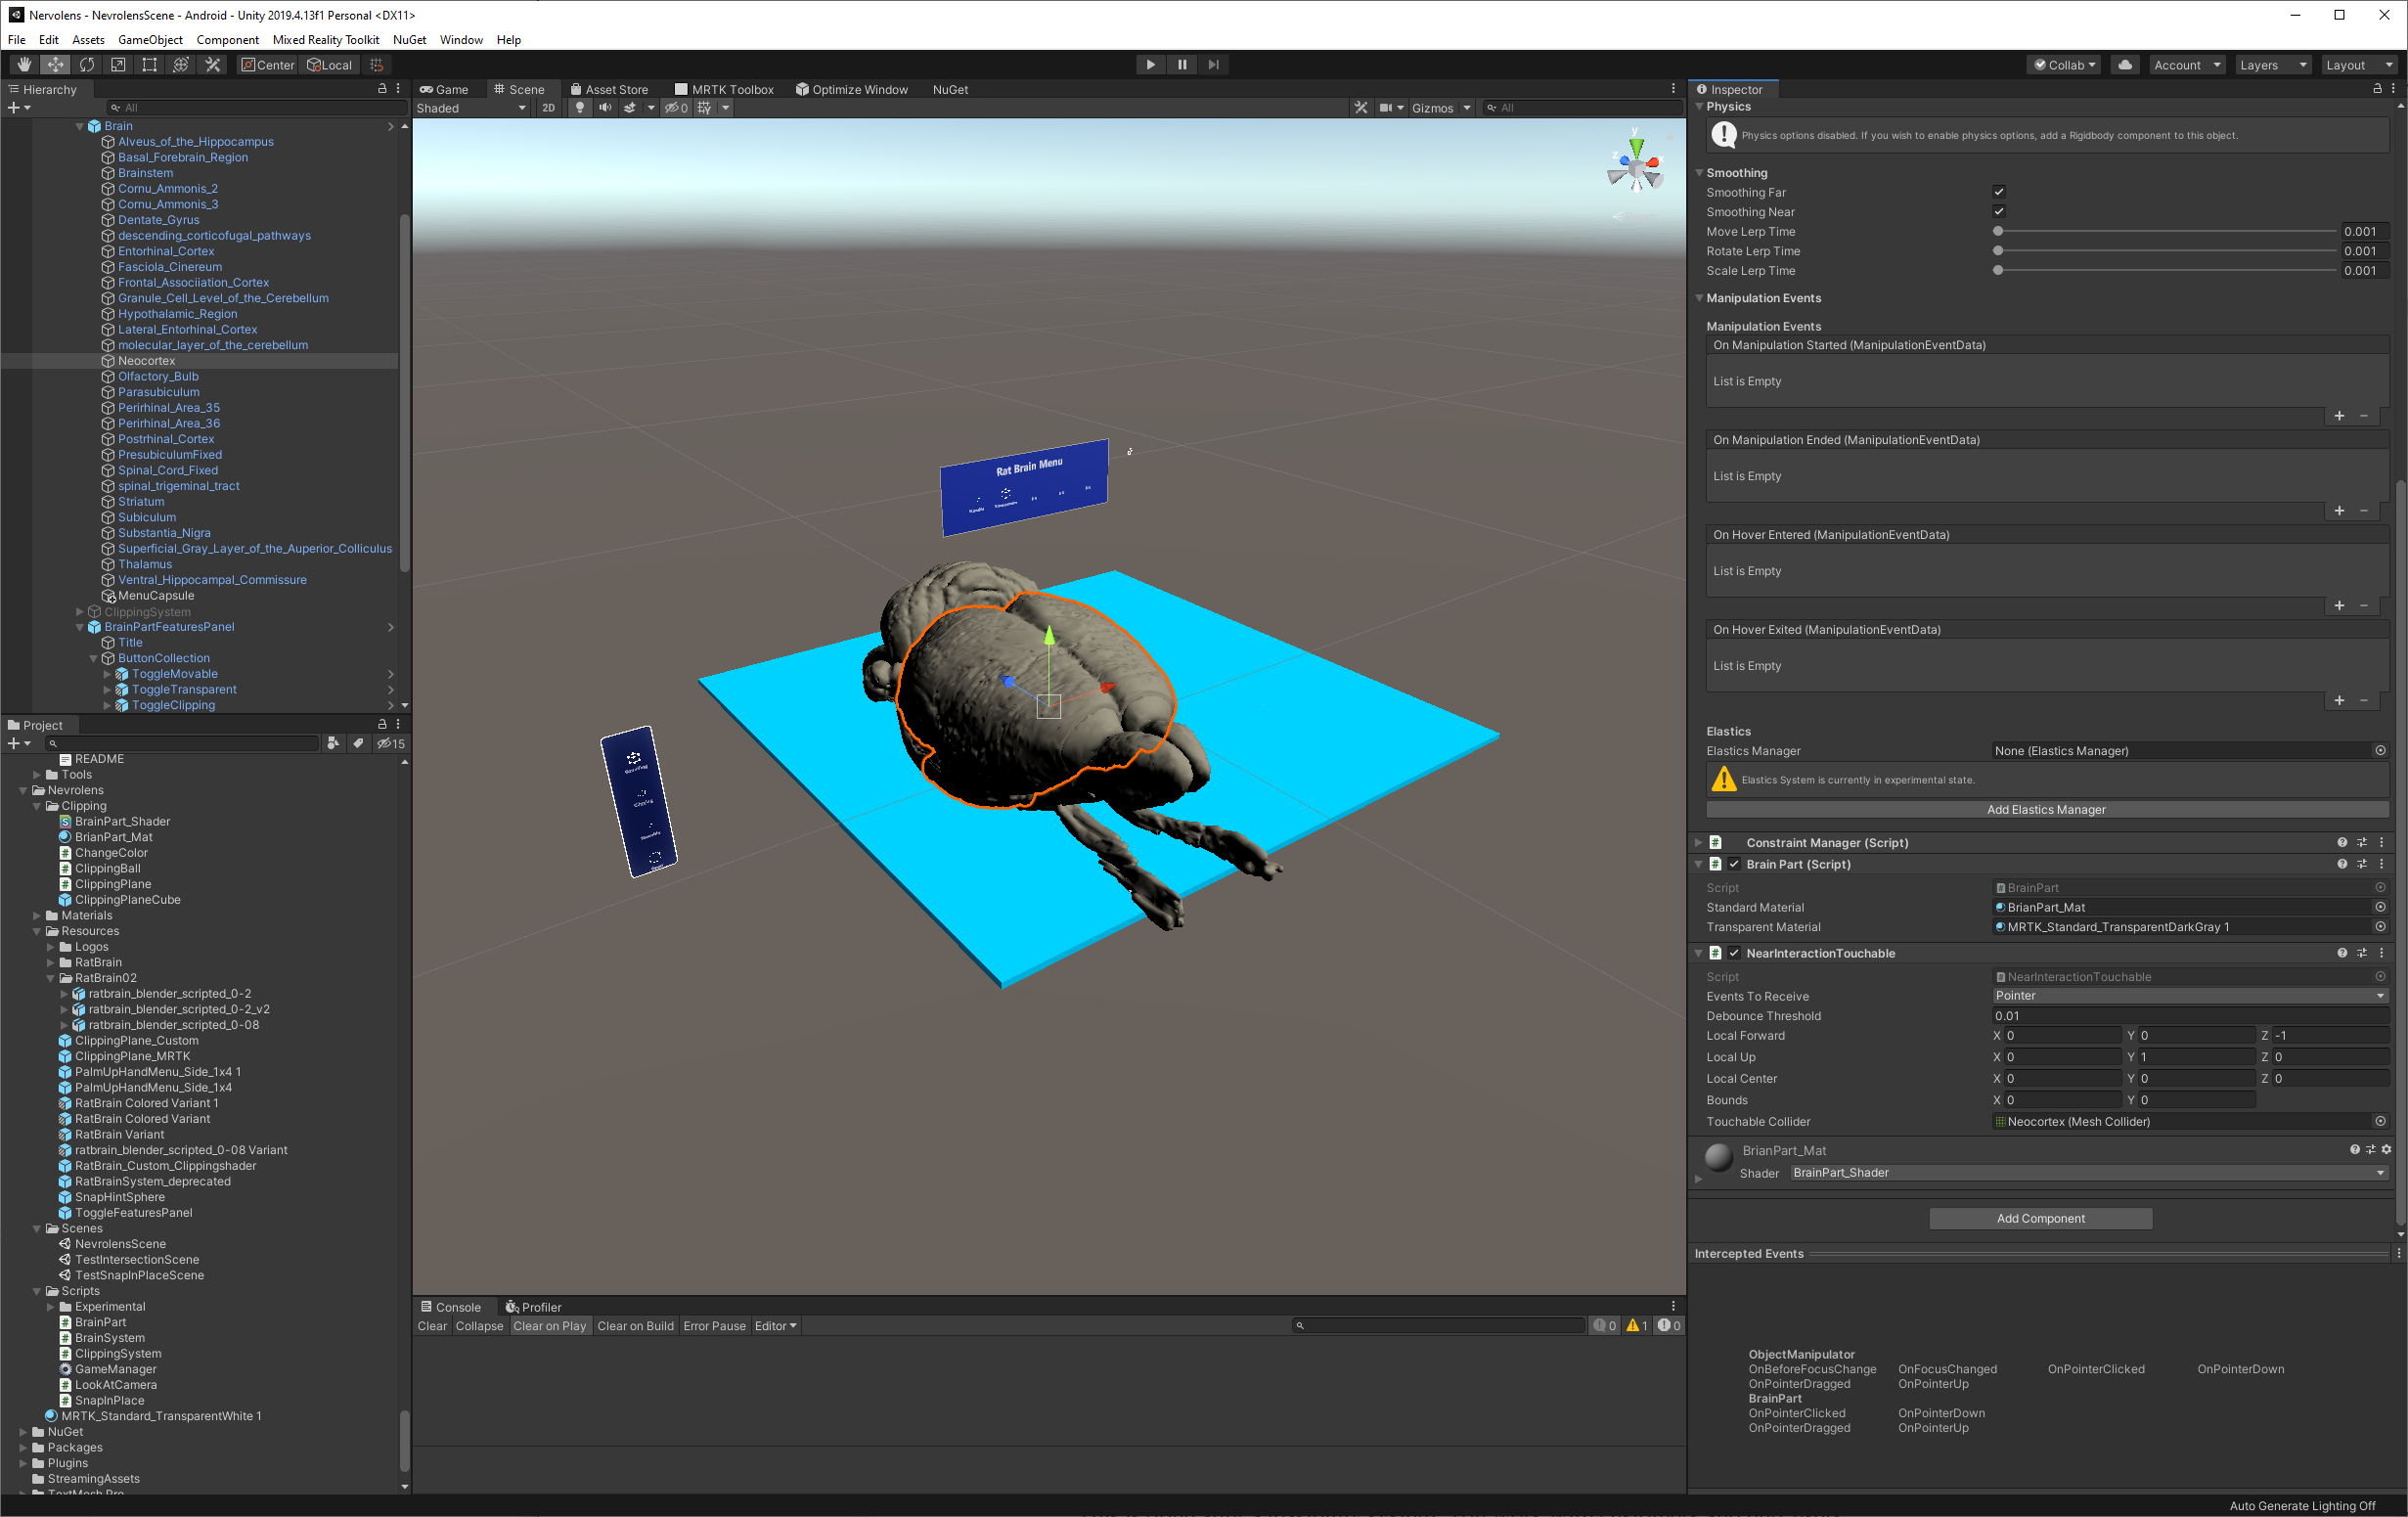
\includegraphics[width=0.8\textwidth]{fig/unity_example.png}
    \caption{Unity 2019.4.13f1 running Nevrolens}
\end{figure}

Unity is a game engine for developing 2D and 3D games. It has grown to become the most popular game engine used by single developers and small development teams because of its ease of use and simple licensing terms for independent developers. Because of its popularity  and ease of use Unity has become a platform for 3D development within more widespread fields than video gaming, such as engineering, moviemaking and architecture. 
Within this project the critical reason for choosing Unity for our 3D development is the exceptional support for the HoloLens product line. As seen in the \autoref{chap:mrtk}, Microsoft has poured resources into developing a "relatively" robust open framework for using Unity to develop for HoloLens. 
Alternatives to using Unity are slim, but one could be to use Unreal Engine, an 3D game engine with great support for VR and AR in general, however the support for HoloLens specific tools like \nameref{chap:mrtk} is limited, Microsoft has a version of MRTK for Unreal, called \href{https://github.com/microsoft/MixedRealityToolkit-Unreal}{MRTK-Unreal}. It seems to be stale however, not having any updates in the last six months in the time of writing.
% An alternative to using Unity wo

\subsection*{Mixed Reality Toolkit}\label{chap:mrtk}
Mixed Reality Toolkit (MRTK) is a open source, Microsoft-driven framework for Mixed Reality (MR) development. In practice it is Microsoft's SDK for HoloLens development, greatly simplifying development related to interaction, user interface and device sensors. As it is a framework for MR in general, it supports other platforms like Android, iOS and VR devices such as HTC Vive and Oculus Rift with OpenVR. 
An alternative to using MRTK would be to us XRTK which is a community-driven fork of MRKT. Thought such a choice would be an exercise of free software principles, it also lends it self to better support for some devices, like the MagicLeap.



\subsection*{Blender}\label{chap:blender}

Blender is a 3D modeling application, it is free open source software and is has a wide set of functionalities for 3D modeling, animation, rendering and optimization. This was chosen because of its free and open availability. 



\subsection*{Photon Unity Networking 2}\label{chap:pun}
Photon Unity Networking 2 (PUN) is the state of the art networking library for Unity. It can manage everything from voice chat to interaction over network. 


\subsection*{Windows Device Portal}\label{chap:wdp}

Windows Device Portal is an web-based application for managing devices running Window, like HoloLens. The HoloLens 2 hosts this application if it's connected to a network, so you can easily log in on the device and manage files, profile application or stream video from it.


\subsection*{Git}\label{chap:git}
% Git flow, Gitmoji, GitKraken, Git gud 
Git is a distributed version control system. Together with hosting on NTNUs self-managed GitLab it enables version control and cloud back-up of the project. While this is the most conventional version control system for any software project, using Git with Unity can be frustrating. 
% There are two main problems with this approach; file sizes and binary changes.
Git is design for projects with only (mostly) small, human-readable text files, like a code base. A Unity project often as huge files, which Git does not support, and relevant changes can happen in binary files, which makes merging impossible. To mitigate this problems the use of Git LFS was needed. It is an extension for Git which enables storages of larger files. Together with enabling only human readable settings in Unity and a long gitignore file, Git with Unity was manageable.
A good alternative to this use of Git is \textit{Unity Collab}, which is Unity's answer to version control, it lack many features found in Git, but would probably be just fine for a project of this scope with a single programmer. However, I like Git very much and find the feature-set of Git to be very helpful. 



\subsection*{GitKraken}\label{chap:gitkraken}
% Kanban and such \\
% Used both / separately for Nevrolens and Project thesis.
GitKraken is a graphical Git management tool. What's more relevant here is its Kanban feature, or GitKraken Boards as their called. This enables synchronization of Kanban tickets and feature branches in Git, and generally makes my life easier.
\begin{figure}[ht]
    \centering
    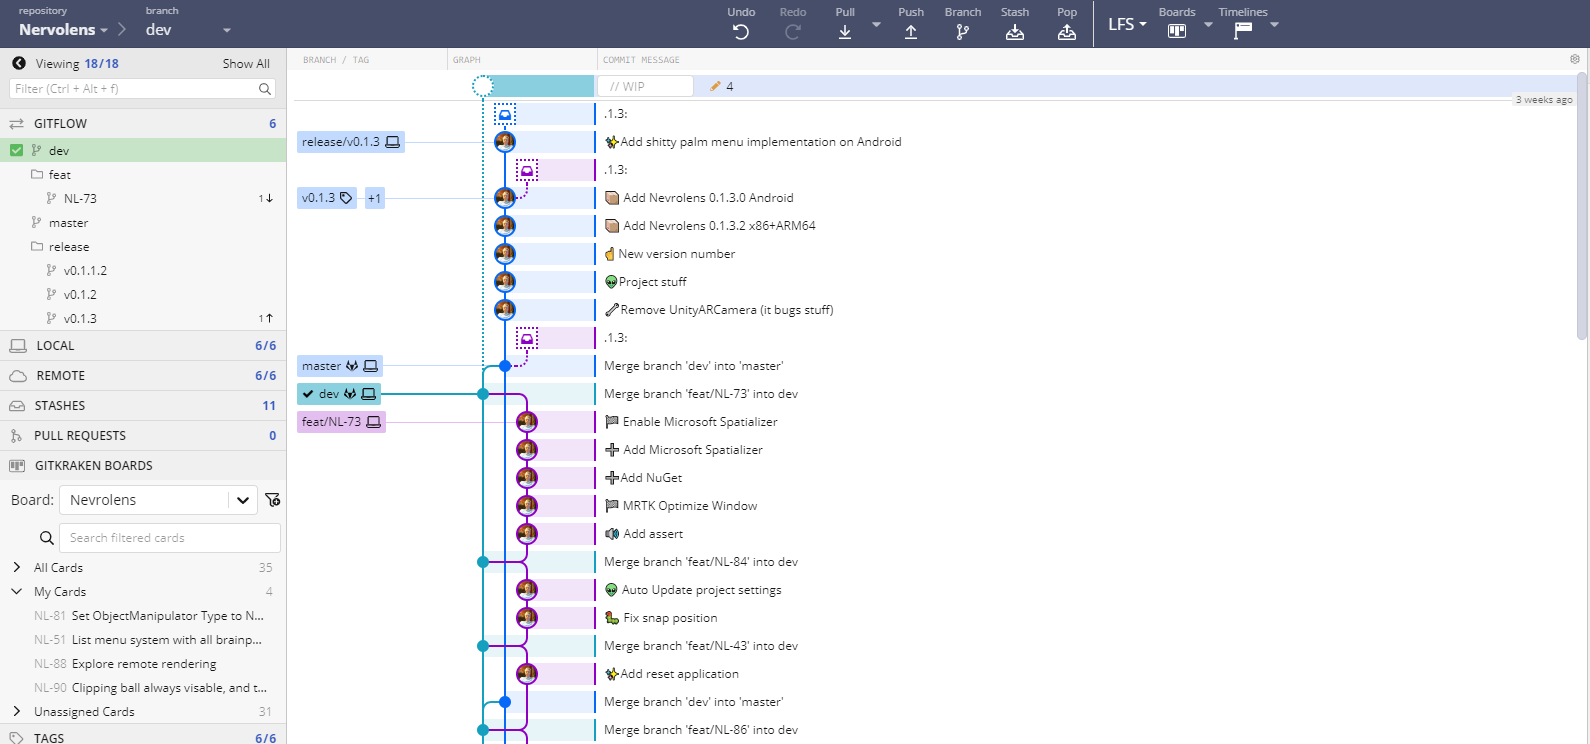
\includegraphics[width=0.8\textwidth]{fig/gitkraken}
    \caption{Git log in GitKraken, on the left you can see synchronized Kanban tickets}
\end{figure}


\section{Related work}

\subsection*{VRVisualizer}\label{chap:vrvis}
\begin{figure}[ht]
    \centering
    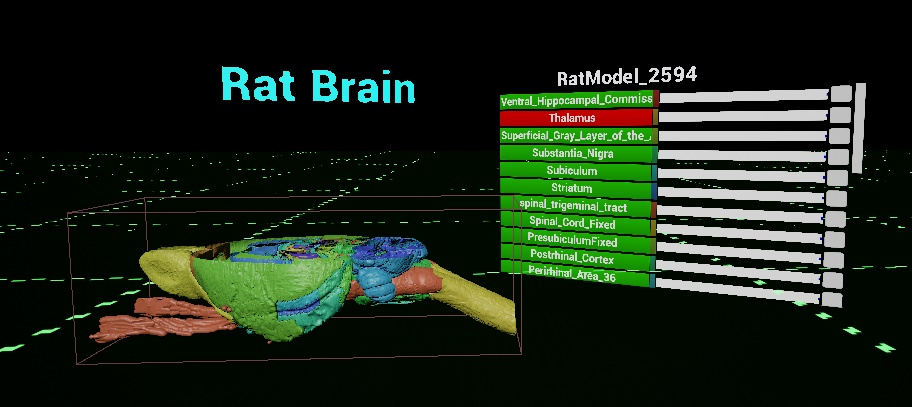
\includegraphics[width=\textwidth]{fig/vrvis_ratbrain.jpg}
    \caption{Cutting operation in VRVisualizer on HTC Vive}
    \label{fig:vrvis}
\end{figure}
VRVisualizer is the name of the research product from the master thesis \citet{Elden2017}. It is a VR application running on the HTC Vive. While its features are similar to the goals of this project, the focus of Eldens project was to develop universal guidelines for scientific visualization in VR. That is far from this projects goals and thus its feature set, relating to interaction and exploration, is quite superficial.


\subsection*{ITK-Snap}

ITK-Snap is an open-source interactive computer application for navigating medical imagery. It is a convectional tool used to display, segment and label 3D neuroanatomical data. It supports a wide array of visual tools which helps in learning about the brain.
However, the fact that it is purely displayed on a two dimensional monitor, means it limits the opportunity of spatial understanding.

\begin{figure}[ht]
    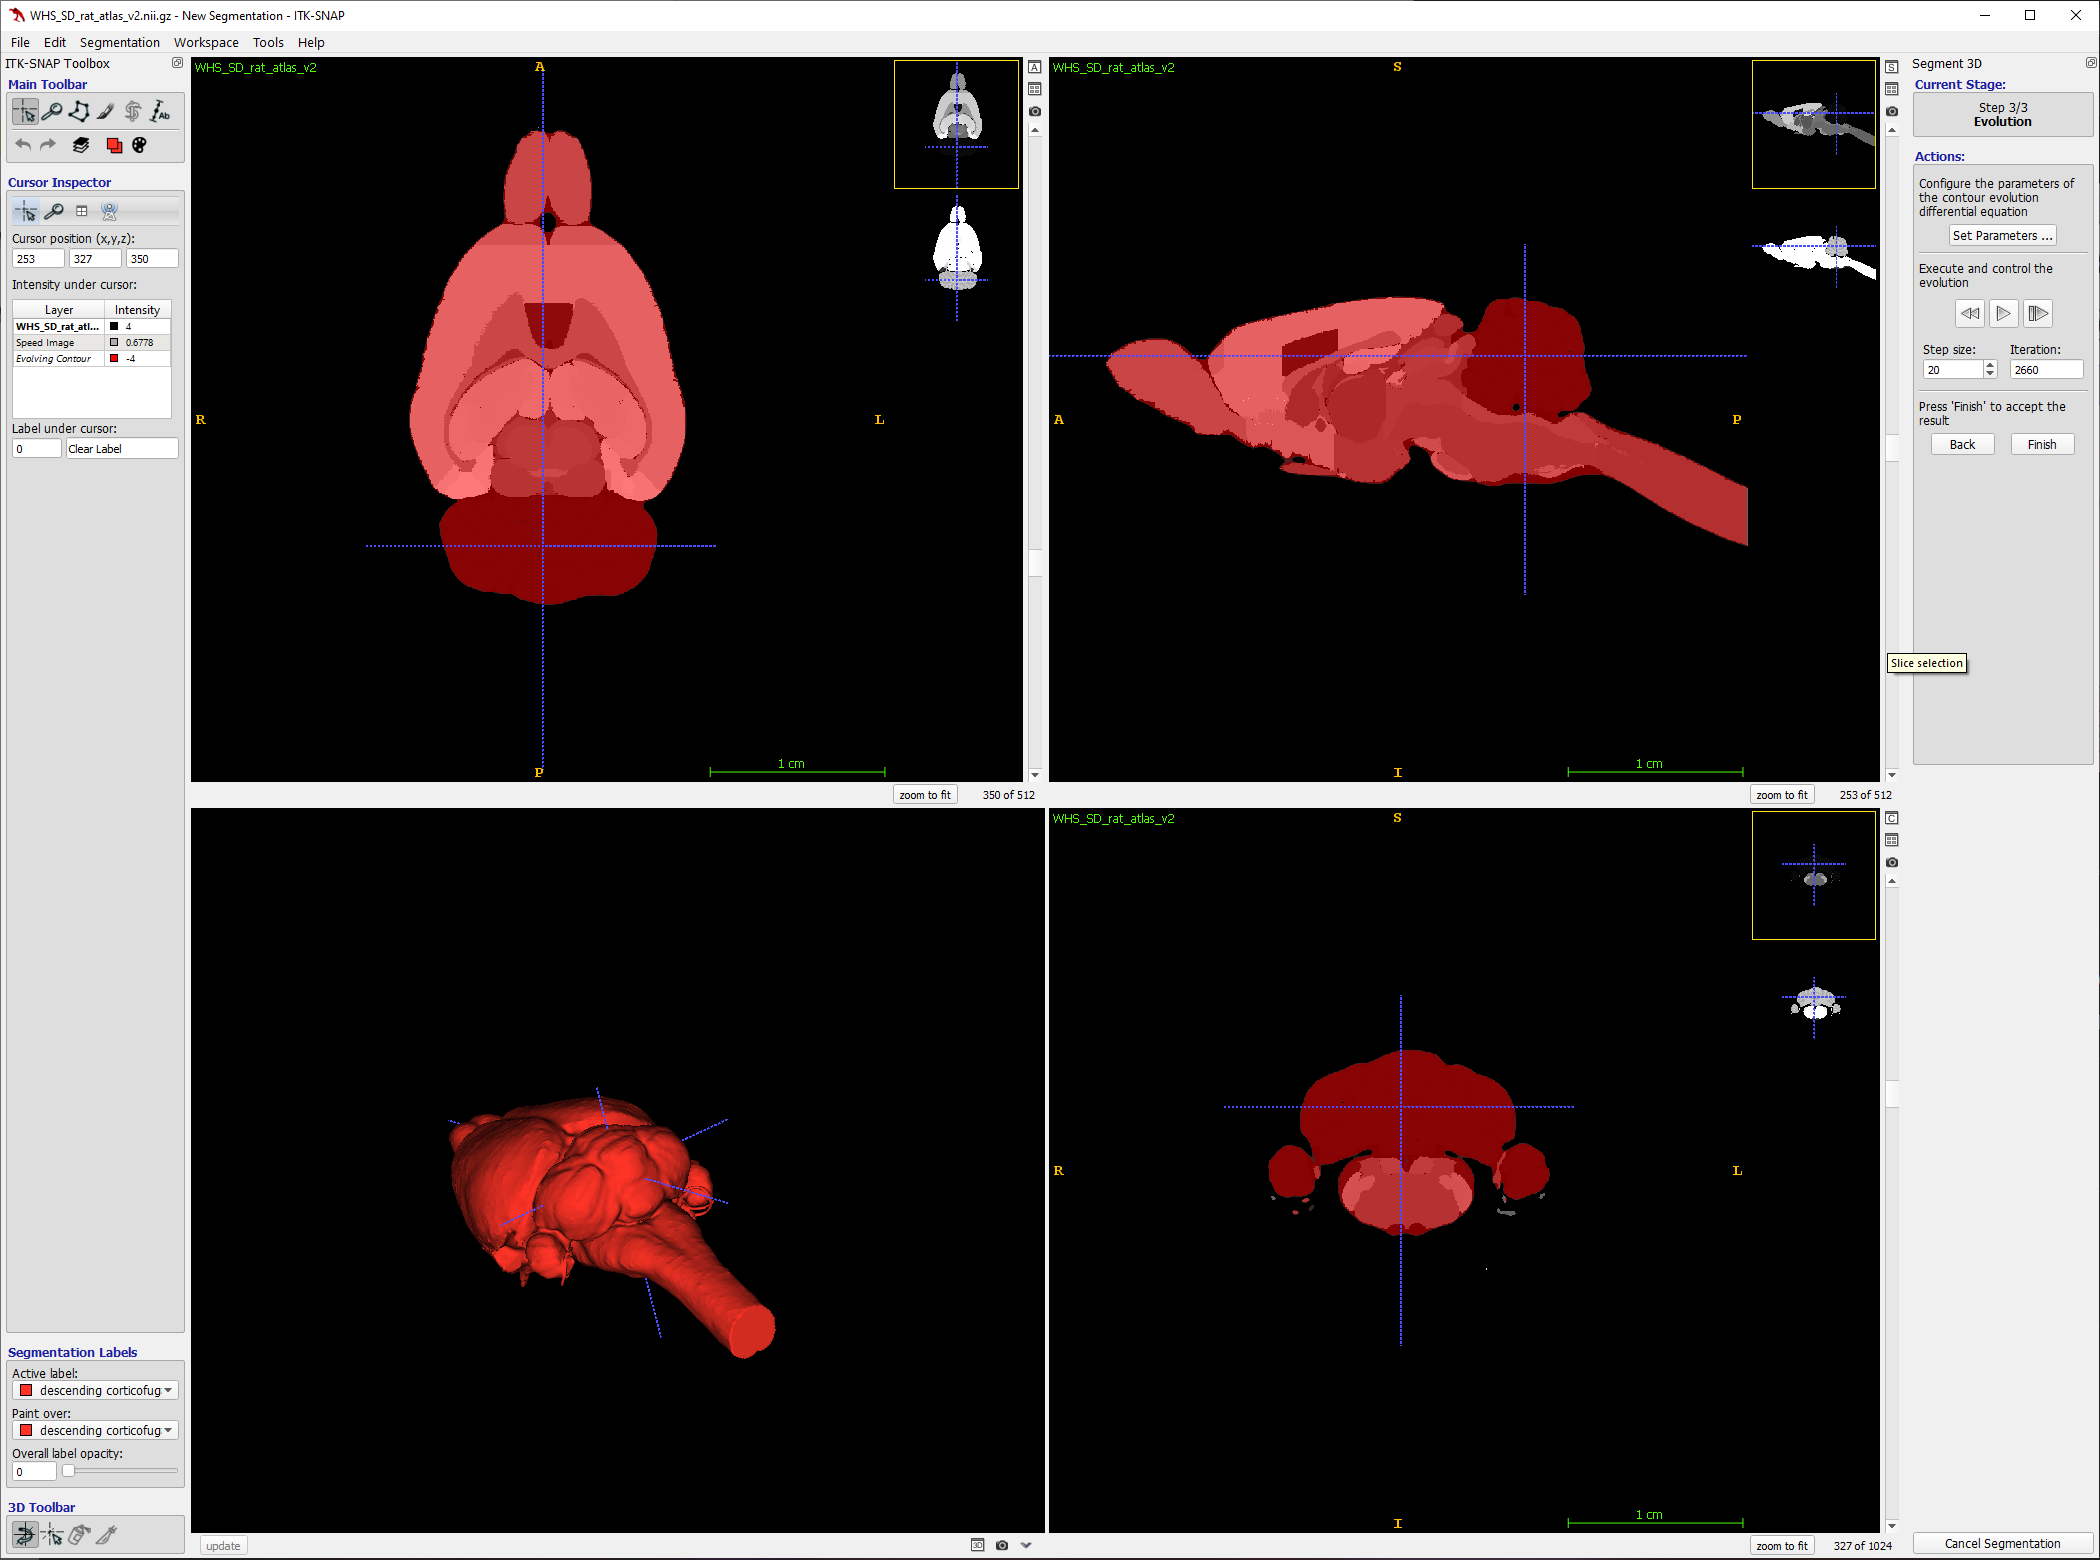
\includegraphics[width=0.5\textwidth]{fig/itk_snap}
    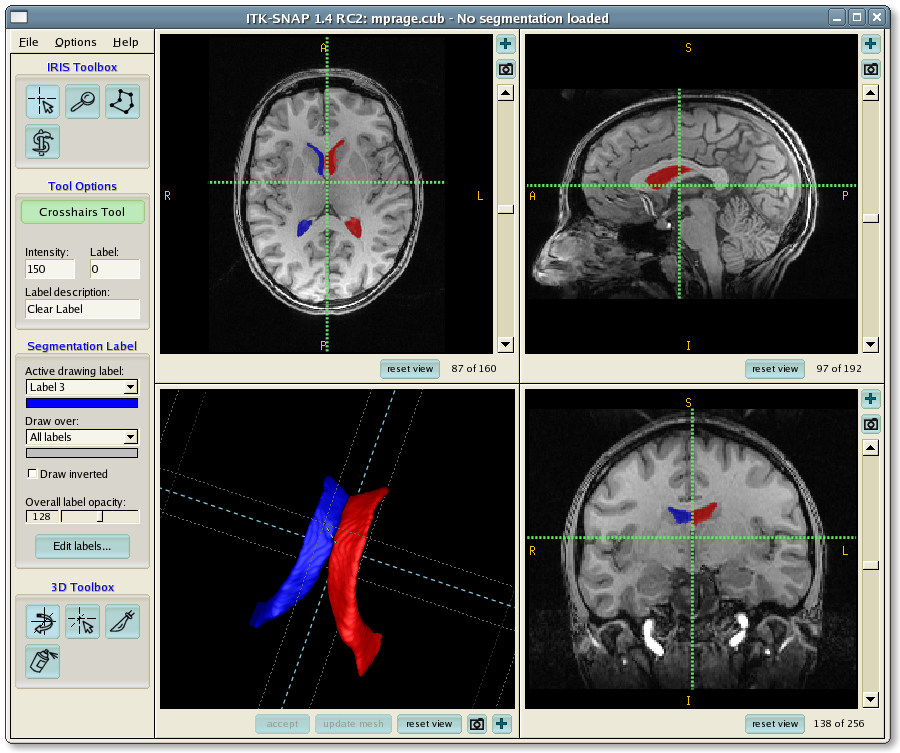
\includegraphics[width=0.5\textwidth]{fig/itk_snap_example}
    \caption{ITK-Snap, Waxholm Space Rat Brain (left), Human brain (right)}
\end{figure}

\subsection*{HoloAnatomy}

HoloAnatomy is a application running on HoloLens, which aims to be a educational tool for anatomy including basic neuroanatomy. \citet{Wish2020} has shown great promise in use of this application for education. While this application is really promising, it lacks some features we would like to focus on. There is no use of mobile devices for collaborative learning. And HoloAnatomy focuses on the macroscopic image of anatomy, and does not go into microscopic detail, which is something this project aims to do. Further, at NTNU and the Kavli Institute research and education using rat brains is normal an thus visualizing it it AR is also a focus.

\begin{figure}[ht]
    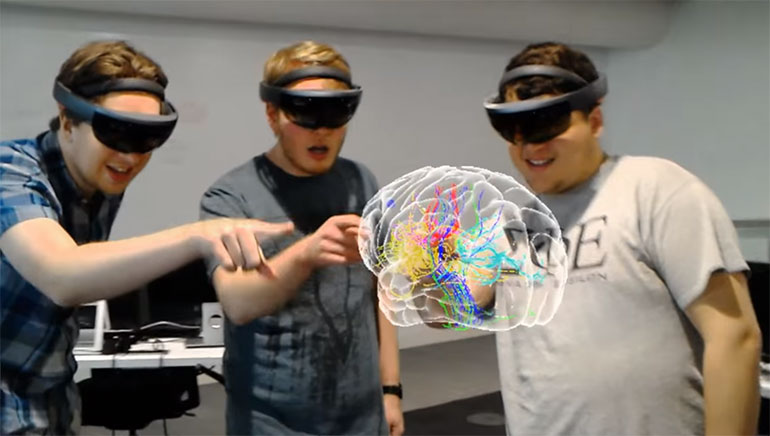
\includegraphics[width=0.5\textwidth]{fig/holoanatomy1}
    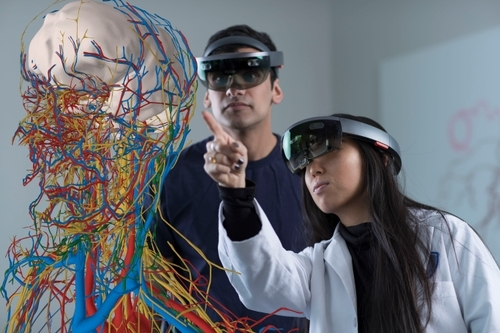
\includegraphics[trim={0 1.76cm 0 0},clip,width=0.5\textwidth]{fig/holoanatomy2}
    \caption{HoloAnatomy}
    
\end{figure}